\documentclass[../main.tex]{subfiles}

\begin{document}

Most \gls{cryoem} image processing suites such as Relion\cite{scheres2021}, Cryosparc\cite{cryosparc}, Cistem\cite{grigorieff2018} and Xmipp\cite{sorzano2021} implement a refinement step in which a 3D model is iteratively improved. This process should converge to a high resolution solution which is compatible with the provided images. 

The input for this step is a large set of noisy images presumably containing the projection of a particle. A rough estimate of the volume is also provided (initial volume). 

Input images are not clean, in fact they have many artefacts. Firstly, they have been ``coloured'' in frequency space by a transfer function known as \gls{ctf}. This transfer function has been estimated in previous steps, so it does not need to be deduced (although it can be fine-tuned). Moreover, the particle is not perfectly centered in the image box. Last but not least, the images contain a vast amount of noise. In fact, the \gls{snr} is in the order of $xx \si{\decibel}$. The \gls{psd} of the noise roughly resembles to pink noise. However, the exact \gls{psd} of the noise is unknown and should also be estimated from data.

Before attempting to reconstruct the 3D structure of the specimen, the projection directions of each of the images need to be deduced in a process known as particle alignment. This is a computationally expensive task and much effort has been put into it to reduce the amount of time expended on this process. 

The alignment process relies on projecting the current volume from multiple perspectives, somewhat mimicking the microscope's behaviour. Then, each of the particle images is searched across all simulated projections, considering in-plane transformations (rotations and translations). The actual similarity metric used for matching varies across the existing solutions. 

Once a best match has been found, the projection parameters of the selected reference image and its best transform can be assigned to the experimental one. This enables using the experimental images to reconstruct a new volume, potentially with a higher resolution. This last volume can be used as the initial volume for the next iteration. This cycle is illustrated in the figure \ref{fig:3:refinement}. 

\begin{figure}[h]
    \centering
    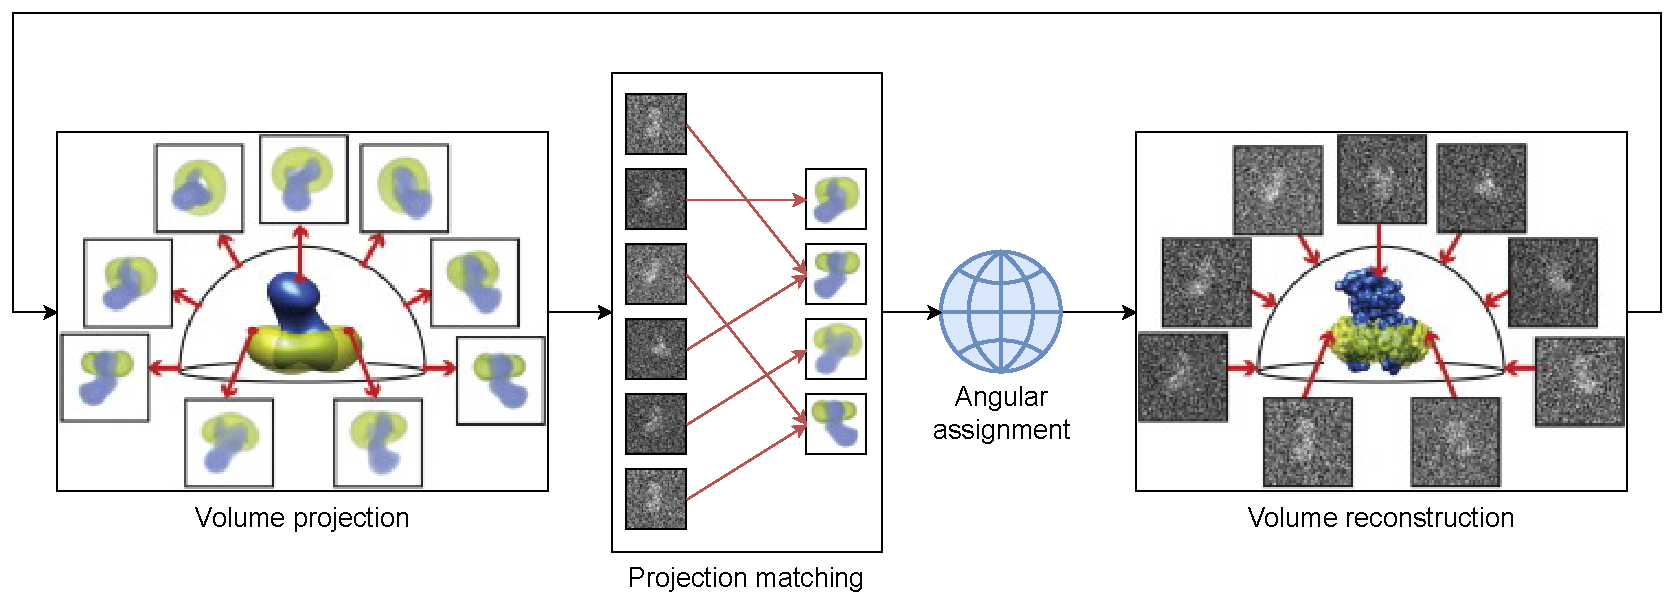
\includegraphics[width=\textwidth]{SPA/refinement}\\
    Images obtained from: \cite{nogales2015}
    \caption{Typical refinement cycle}
    \label{fig:3:refinement}
\end{figure}

\subsection{Projection gallery generation}
The projection gallery represents a set of ``views'' of the input volume from relevant directions. This collection of images is generated by projecting the initial volume in the same way that a \gls{tem} microscope would do. This enables performing comparisons between experimental and generated images. 

\subsubsection{Projection procedure}
\Gls{tem} microscopes fire a electron beam through the sample and capture the ``shadow'' of its electron density. In other words, areas where the beam encounters electrons will appear dim. This process is illustrated in the figure \ref{fig:3:projection}. Nevertheless images are usually complemented so that bright areas relate to the presence of matter.

\begin{figure}[h]
    \centering
    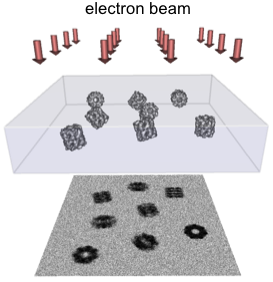
\includegraphics[width=.5\textwidth]{SPA/projection_reconstruction/acquisition}\\
    Images obtained from: \cite{greg}
    \caption{TEM image acquisition}
    \label{fig:3:projection}
\end{figure}

This behaviour is mathematically known as the X-Ray transform, which is a particularisation to 3 dimensions of the Radon's transform. As described in the equation \ref{eq:3:xray}, this transform consists in computing the integral across a set of parallel lines normal to the projection plane.

\begin{equation}\label{eq:3:xray}
    Xf(L) = \int_L f
\end{equation}

This computation can be significantly accelerated using the Fourier Central Slice Theorem. This theorem states that projecting a $N$-dimensional function to $N-1$ dimensions and then taking its \gls{ft} is equivalent to computing the $N$-dimensional \gls{ft} and then extracting the central hyperplane normal to the projection direction. This equivalence is shown in the figure \ref{fig:3:3dfourier}. Therefore, a set of projections can be generated by extracting 2D planes from the 3D \gls{ft} of the input volume and then computing their \gls{ift}.

\begin{figure}[h]
    \centering
    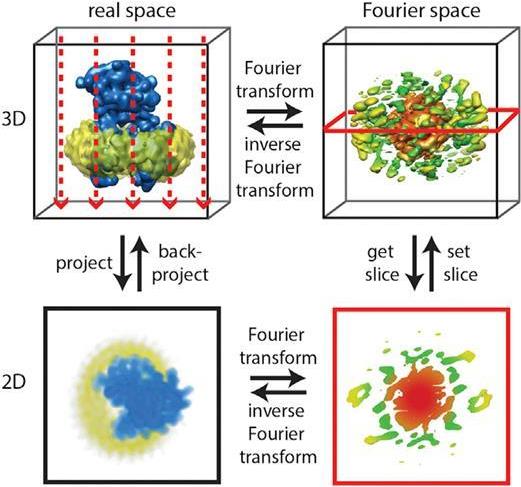
\includegraphics[width=.5\textwidth]{SPA/3d_fourier_reconstruction}\\
    \cite{nogales2015}
    \caption{Fourier Slice Theorem illustration for 3D}
    \label{fig:3:3dfourier}
\end{figure}

Note that when using this approach, only one 3D \gls{fft} is computed, and then for each projection direction, a 2D central slice is extracted from it, which contains the 2D \gls{ft} of the projected image. More often than not, the following steps are performed in Fourier space, so computing the \gls{ift} of the slices is not needed.

\subsubsection{Projection angle generation}
Regarding the projection angles, these are selected so that they are as homogeneously distributed as possible. Most current refinement packages such as Relion inherit the \gls{healpix} distribution from astronomy. Some of these angle distributions are shown in the figure \ref{fig:3:healpix}.

\begin{figure}[h]
    \centering
    \begin{subfigure}[b]{0.33\textwidth}
         \centering
         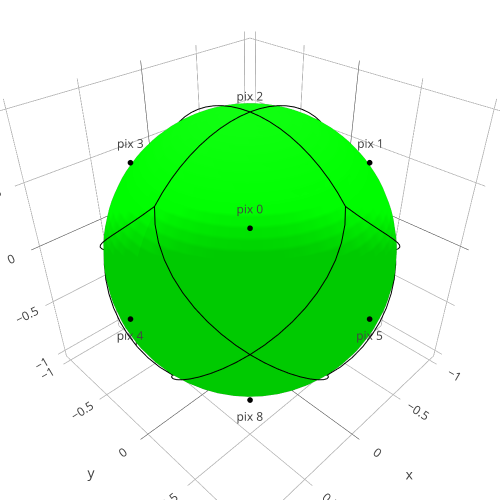
\includegraphics[width=\textwidth]{healpix/1}
         \caption{Nside 1}
         \label{fig:3:healpix:1}
    \end{subfigure}
    \begin{subfigure}[b]{0.33\textwidth}
         \centering
         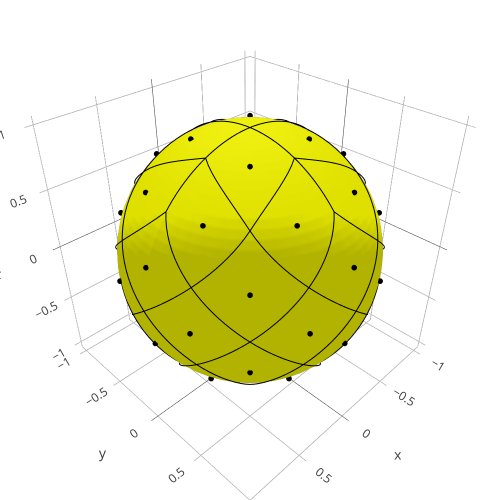
\includegraphics[width=\textwidth]{healpix/2}
         \caption{Nside 2}
         \label{fig:3:healpix:2}
    \end{subfigure}
    \\
    \begin{subfigure}[b]{0.33\textwidth}
         \centering
         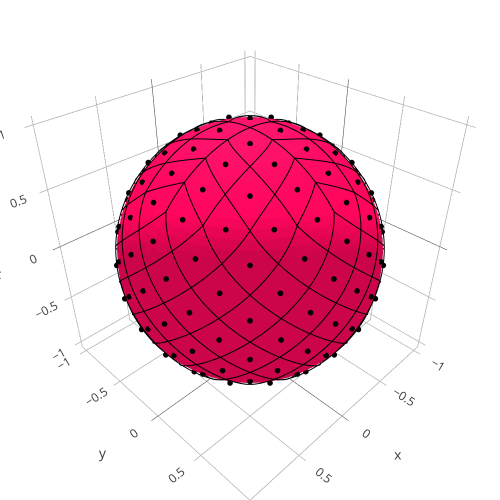
\includegraphics[width=\textwidth]{healpix/4}
         \caption{Nside 4}
         \label{fig:3:healpix:4}
    \end{subfigure}
    \begin{subfigure}[b]{0.33\textwidth}
         \centering
         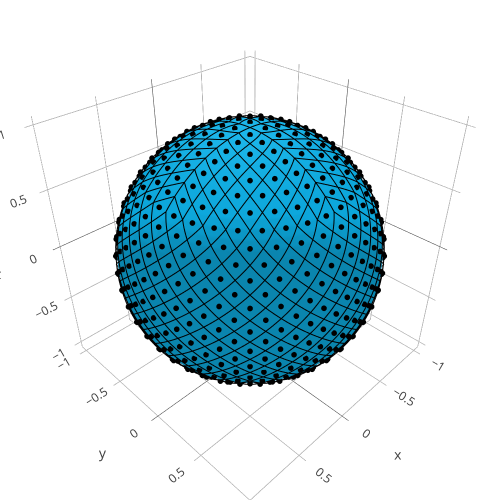
\includegraphics[width=\textwidth]{healpix/8}
         \caption{Nside 8}
         \label{fig:3:healpix:8}
    \end{subfigure}\\
    Images obtained from: ??
    \caption{HEALpix distribution examples}
    \label{fig:3:healpix}
\end{figure}

Obviously, the angular sampling rate will condition the angular accuracy of the angular assignment. In theory, when no noise is present, the angular assignment error will have a uniform distribution from $0$ to $\Delta$, where $\Delta$ is the angular sampling step. This distribution has a mean value of $\frac{\Delta}{2}$. Therefore, as the target resolution of the reconstructed volume rises, the angular sampling rate also needs to be increased, so that the angular error decreases. Typical sampling rates provided by \gls{healpix} are shown in the table \ref{tab:3:healpix}.

\begin{table}[h]
\centering
\begin{tabular}{|l|c|c|}
\hline
HEALpix order & $\Delta$ ($\si{\degree}$) & N                           \\ \hline
0             & 58.6                      & 12                          \\ \hline
1             & 29.3                      & 48                          \\ \hline
2             & 14.7                      & 192                         \\ \hline
3             & 7.33                      & 768                         \\ \hline
4             & 3.66                      & 3072                        \\ \hline
5             & 1.83                      & 12288                       \\ \hline
6             & 0.55                      & 49152                       \\ \hline
7             & 0.28                      & 196608                      \\ \hline
8             & 0.14                      & 786432                      \\ \hline
\end{tabular}
\caption{HEALpix angular sampling}
\label{tab:3:healpix}
\end{table}


Sometimes the particle of interest presents some symmetry. In those cases, only a patch of projection angles belonging are relevant, as the rest is composed of repetitions of the same patch.

Moreover, when there is faith in the accuracy of a prior angular assignment, we can perform a local search. This means that for each particle, only projections in its neighbourhood are searched. In fact, as shown in the table \ref{tab:3:healpix}, global searches become impractical for very tight angular samplings, as the amount of reference images increases quadratically. Although local searches reduce the reference dataset, they involve the risk of falling into local minimas.

\subsection{Projection matching and angular assignment}
Each of the input particles needs to be searched across the images generated in the prior section, also considering all possible in plane transformations (rotations and shifts). Similarly to the gallery generation step, this in-plane transform explocation can be local, only considering rotations and shifts near the previous one, with the same associated local minima risk.

Additionally, the \gls{ctf} needs to be considered. Experimental images have been ``coloured´´ with a characteristic transfer function induced by the microscope. As opposed to this, the reference gallery was generated artificially without considering any frequency response. Therefore, this transfer function needs to be addressed before attempting to compare images to one another. Most current implementations choose to filter the reference images with the experimental's estimated \gls{ctf}. Note that the \gls{ctf} may vary from particle to particle. Therefore, for each particle, the \gls{ctf} needs to be re-applied to the reference gallery.

In essence, this step can be seen as a \gls{knn} problem with $k=1$. This means that we have a large set of images composed of all the projections of the current volume and its in plane transformations. For each experimental image we want to find the most similar one, this is, the image which minimises some distance metric.

The problem can be mathematically expressed with the expression \ref{eq:3:minimization} where $C$ is the estimated \gls{ctf} of the experimental image $I_{exp}$. $\Phi$ is a projection $\mathbb{R}^3 \mapsto \mathbb{R}^2$. Finally, $V$ is the reference volume. The actual distance function used depends on the implementation. All of $C$, $V$ and $I_{exp}$ remain constant for a given search. Therefore, only the projection parameters regarding $\Phi$ need to be optimised.

\begin{equation}\label{eq:3:minimization}
    \min_\Phi \text{dist}(C\Phi V, I_{exp})
\end{equation}

This projection is usually characterised by the following parameters:

\begin{itemize}
    \item \textbf{Euler angles}
    \begin{itemize}
        \item \textbf{Tilt}: Equivalent to latitude in the projection sphere
        \item \textbf{Rotation}: Equivalent to longitude in the projection sphere
        \item \textbf{Psi}: In-plane rotation of the projection
    \end{itemize}
    \item \textbf{In-plane shift}
    \begin{itemize}
        \item \textbf{Shift X}: In-plane shift in the $X$ axis
        \item \textbf{Shift Y}: In-plane shift in the $Y$ axis
    \end{itemize}
\end{itemize}

However, Euler Angles, although intuitive, they are tricky to manipulate due to gimbal lock. Therfore, some implementations prefer to represent the projection parameters using a affine transformation matrix. This means that $3\times4$ matrix is needed to store this information. This matrix represents how the reference volume should be transformed so that the target projection is obtained simply projecting in the $Z$ direction\cite{delarosa2016}.

\subsubsection{Distance metrics}

\subsection{3D reconstruction}

\subsection{Post-processing}

\subsection{Multi-reference refinement}
The refinement algorithms rely on the assumption that all input particles belong to the same structure. However, this is not always true, as the dataset might be heterogeneous. This heterogeneity can be either discrete or continuous. 

The continuous heterogeneity relates to flexible macromolecules. These macromolecules have a certain amount of freedom to deform. Therefore, when projecting them, no single conformation can be attributed to the dataset. This is a novel field which is under study.

Contrary to this, discrete heterogeneity involves a discrete amount of conformations in the dataset. For instance, a biologist may want to test how a particular ligand binds to the protein. In that case, it is reasonable to consider that some of the input particles may come from a structure with the ligand attached, whilst some others won't have it.

The most common way to solve discrete heterogeneity is to generalise the refinement algorithm to $N$ volumes. This is done by enabling multiple projection gallery inputs to the projection matching stage. Here, not only the projection parameters need to be considered, but also the reference volume. Then, each of the volumes can be reconstructed with the particles that were classified as such.

\end{document}
